\chapter{Introducción}

Mi primer contacto con la informática fue a finales de los años ochenta. Un buen día mi padre apareció en casa con una caja negra y alargada que contenía un misterioso teclado que se enchufaba a la tele. En ese mismo teclado se introducía una cinta de cassette como las que poníamos para escuchar música y tras esperar un rato, que ahora nos parecería una eternidad, podíamos empezar a aporrear el teclado para llevar a Phantomas (ver figura \ref{fig:phantomas}) de pantalla en pantalla mientras íbamos esquivando enemigos y activando las palancas que abrirían la caja fuerte de la mansión que íbamos a robar.


\begin{figure}[h!]
\centering
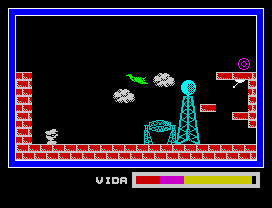
\includegraphics{../screenshots/phantomas-sp1}
\caption{Phantomas (© 1986 Dinamic)}
\label{fig:phantomas}
\end{figure}

\bigskip
Todavía faltaba mucho tiempo para que aprendiera lo que era una interfaz (aún no había aprendido ni tan siquiera a leer) pero ya sabía interpretar algunas letras, curiosamente las que tenían pintadas las teclas OPQA\footnote{En los primeros ordenadores que aparecieron en España en la década de los 80 esta era la combinación de teclas que tenían predefinidos la mayoría de los juegos siendo OP las teclas para moverse de izquierda a derecha y QA para hacerlo de arriba a abajo.}.

\bigskip
Según fui creciendo aprendí a leer y escribir y también a reconocer unos códigos que aparecían al final de las revistas que compraba mi hermano que se llamaban POKES\footnote{Instrucción en lenguaje BASIC que graba un valor en una determinada dirección de memoria.}, estos códigos hacían que, introduciéndolos a la hora de cargar el juego, pudiera tener vidas infinitas, la habilidad de atravesar paredes o la capacidad de ser invisible a los enemigos. Estos trucos permitían a un niño torpe a los mandos, como lo era yo, el poder terminar los dificilísimos juegos de la época.

\bigskip
Pasaron algunos años y ya en el colegio muchos amigos tenían consolas de videojuegos en las que metías un cartucho e instantáneamente estabas jugando a juegos increíbles con una paleta de colores que raro era que no provocara ataques epilépticos. Mientras mis amigos solo tenían que introducir el cartucho y empezar a jugar yo tenía que esperar 5 interminables minutos mientras escuchaba sonidos estridentes y cruzar los dedos por que no apareciera el fastidioso TAPE ERROR que se podía intentar solucionar girando un tornillo llamado 'azimut' con un destornillador que curiosamente aún poseo. 

\bigskip
Quizá fue ahí donde empecé a sufrir los problemas de la usabilidad, yo girando un tornillo sin saber a ciencia cierta el por qué y mis amigos el mayor problema que tenían era que a veces tenían que dar un soplido fuerte a la ranura del cartucho.

\bigskip
Mucho mas tarde entró en mi casa un flamante Pentium 166 MMX con Windows 95 OSR2 y esto era otra cosa, tenía ventanas, podía escribir documentos con formato y el primo de un conocido tenía un programa te marcaba en rojo los errores ortográficos de los trabajos del colegio. De hecho ese mismo tío tenía un CD llamado Encarta donde había toda una enciclopedia metida dentro, solo tenías que escribir una palabra y al momento aparecía su definición con fotografías y todo.

\bigskip
Estábamos ya a mediados de 1996 y se empezaba a hablar de Internet, era como aquella Encarta pero sin CD, el futuro nuevamente había llegado y todo el dinero invertido en una grabadora de CD se iba al garete, junto con las horas mantenidas cruzando los dedos y sin tocar el ordenador para que fallara la grabación, todo estaba en Internet, y si no estaba ahí poco tardaría en estarlo.

\bigskip
Así que cogí los ahorros de mi paga semanal y me compré un módem para puerto serie de 33.000 Baudios de segunda mano. Aún hoy no tengo claro lo que significaba la palabra baudio. Conecté el módem metí uno de los múltiples de CDs de conexión a Internet que regalaban por aquel entonces con las revistas, le di a conectar y ahí estaban de nuevo las largas esperas escuchando ruidos estridentes igual que unos años antes.

\bigskip
A base de curiosear como buen aspirante a ingeniero vi escondido en las opciones una casilla que decía 'Silenciar altavoz', ¿como podía ser que millones de personas estuvieran soportando esos ruidos estridente para conectarse por no saber marcar una casilla? Algo raro pasaba ya que la opción estaba ahí pero nadie la pulsaba.

\bigskip
Pasaron los años, los sistemas se fueron haciendo mas complejos y me di cuenta que según más opciones tenían los dispositivos más perezosos se volvían los usuarios. Mi vecino sin ir más lejos por no configurar su televisor tenía TVE2 en el canal 4 de su televisor ¿era yo el único que encontraba eso chirriante? Quizá no, pero como he ido descubriendo hay diferentes tipos de personas, están los que pueden pasar meses alumbrando el pasillo con el teléfono móvil y los que simplemente llegan y cambian la bombilla. 

\bigskip
Por eso creo que es nuestro deber como ingenieros, ya que tenemos la capacidad de detectar necesidades de las personas y ponerles solución, ya que tenemos el conocimiento y la capacidad de cambiar el mundo. Podemos dejar silenciado por defecto el volumen del altavoz de un módem o bien podemos inventar una bombilla que nos avise de cuántas horas de vida le quedan.

\bigskip
Y por encima de todo, tenemos la capacidad de hacer sencillas las cosas más complejas que es la premisa básica de la usabilidad. No le puedes pedir a tu madre que entienda la incongruencia de pasarte una foto de tu sobrina en e-mail con un documento de Word adjunto y la foto pegada dentro de dicho documento, tienes que ponérselo fácil para que no haga esas barbaridades.

\bigskip
Por eso es tan importante que los que tenemos los conocimientos los invirtamos en ayudar a mejorar los interfaces. Una gran parte de los usuarios no se va a dar cuenta de los problemas de usabilidad ya que muchas veces dicha usabilidad es subconsciente.

\section{Motivación}

Como ya sabemos Internet ha tenido un carácter académico desde prácticamente su nacimiento y por ello las mayores innovaciones y casi todo su enfoque ha salido de estos ámbitos previos a la democratización de la red y el acceso global a Internet. Es impensable concebir hoy día la enseñanza sin hacer uso de Internet y puede que en un futuro no muy lejano la totalidad de la enseñanza se imparta a través de la red.

\bigskip
Pero un uso tan generalizado es inconcebible sin una interfaz adecuada que sea amigable, sencilla e incluso atrayente y es por eso que muchas empresas gastan millones de dólares en mejorar las interfaces. 'La usabilidad ha venido para quedarse' \cite{jakonielsen}.

\bigskip
Tras la implantación definitiva de la plataforma \textbf{Prado2} por parte de la \textit{Delegación de la Rectora para la Universidad Digital} se han venido sucediendo críticas por parte tanto de alumnos como profesores a las carencias de la plataforma, esto, junto a los insuficientes recursos con los que cuenta el CEVUG para dar un servicio adecuado ha hecho que una plataforma potente y consolidada como es moodle genere rechazo ya que como bien apuntaba Steve Krug: 'Si un sistema no es usable nadie lo querrá usar' \cite{stevekrug}


\section{Estructura del proyecto}


\bigskip
Antes de pasar a detalles más técnicos, me gustaría detallarte lo que te vas a encontrar en este proyecto:

\begin{itemize}
  \item En el \textit{capítulo 1} (\textbf{Introducción}), vas a encontrar el texto que estas leyendo ahora mismo así como una breve historia de las plataformas utilizadas por la Universidad de Granada.
  \item En el \textit{capítulo 2} (\textbf{Objetivos}), detallo de forma algo más concreta los objetivos determinados que se quieren cumplir con este proyecto.
  \item En el \textit{capítulo 3} (\textbf{Metodología}), la planificación y desarrollo de cada uno de los analisis del proyecto.
  \item En el \textit{capítulo 4} (\textbf{Resultados}), detallar todos los resultados obtenidos.
\end{itemize}

\bigskip
Una vez estén realizadas las partes descriptivas y de resultados quedarán solo por añadir la parte final; el \textit{capítulo 5} (\textbf{Conclusiones}) en el que se indicarán las diferentes conclusiones a las que se han llegado así como las recomendaciones tanto de carácter urgente como opcionales.

\bigskip
Para finalizar se incluye un anexo con una selección de los comentarios dados a la encuesta así como el código fuente de los scripts desarrollados.

\section{Historia de las plataformas online de la UGR}

Cuando en el año 2013 comencé mis estudios en la Universidad de Granada me sorprendió el encontrarme con varias plataformas de docencia online, prácticamente una para cada departamento y todas ellas tenían puntos buenos y puntos a mejorar.

\bigskip
En mi segundo año se estaba empezando a implantar Prado2 que venía a resolver el problema de la fragmentación, como ya hemos dicho cada profesor era libre de elegir el sistema que más le gustara pero, a cambio de esta libertad, los alumnos teníamos que aprender a usar todas y cada una de las distintas plataformas.

\bigskip
Quizá no todos los estudiantes de la UGR han tenido que lidiar con esta situación, ya que compañeros de otras facultades sólo han conocido el Tablón de Docencia y a lo sumo SWAD antes de pasar al nuevo Prado2, pero los estudiantes de la ETSIIT, por el carácter de los estudios que tenemos si hemos sido 'conejillos de indias' de todas estas plataformas.

Quisiera agradecer a los responsables de las diferentes departamentos su ayuda a la hora de conocer la historia de cada una las plataformas.

\subsection{Tablón de docencia}

Fue desarrollado por el CSIRC pero, aunque hemos intentado ponernos en contacto con ellos para conocer la historia de esta plataforma, no hemos recibido respuesta.

\subsection{SWAD (Sistema Web de Apoyo a la Docencia)}

Año de publicación: 1999\\

Desarrolladores principales: Antonio Cañas Vargas\\

Lenguajes de programación utilizados: C\\

\bigskip
La primera versión de SWAD apareció en septiembre de 1999. A partir de 2005 comenzó a extenderse su uso en la Universidad de Granada. La aplicación fue liberada en enero de 2010 bajo licencia GNU Affero General Public License, versión 3.
\bigskip
En 2010 el sistema era usado por 1.100 profesores y 35.000 estudiantes. En 2011 la cantidad ascencía a 2.000 profesores y 60.000 estudiantes en 2.800 asignaturas.

\bigskip
En febrero de 2016 la instalación de SWAD en la Universidad de Granada albergaba 419 titulaciones (incluyendo grado y posgrado) con 7114 asignaturas, 110057 estudiantes y 3304 profesores.

\bigskip
SWAD está disponible actualmente en 9 idiomas y se utiliza en la Universidad de Granada y en el portal OpenSWAD.org.

\subsection{PRADO}

Año de publicación: 2014\\

Desarrolladores principales: Emilio Arjona Heredia\\

Lenguajes de programación utilizados: PHP\\

\subsection{DECSAI}

Año de publicación: 2004 la primera versión y 2010 la segunda que corresponde casi exactamente con la actual.\\

Desarrolladores principales: Pablo Orantes Pozo y Miguel García Silvente\\

Lenguajes de programación utilizados: PHP\\

\bigskip
El desarrollo de esta plataforma web ha tenido tres etapas: 
La versión 3.0 disponible a partir de finales de 2013 emplea la plantilla institucional facilitada por la Oficina Web de la Universidad de Granada y es realizada por Pablo Orantes Pozo bajo la dirección de Miguel García Silvente.

\bigskip
La versión 2.0 corresponde a un rediseño y programación casi completo realizado por Pablo Orantes Pozo bajo la dirección de Miguel García Silvente.

\bigskip
La versión 1.0 (2004-2009) se realizó bajo la coordinación de Miguel García Silvente, Francisco G. Raúl Pérez Rodríguez y Gracia Pérez López.

\bigskip
Las tareas de programación de la versión 1.0 fueron realizadas por: Carlos Cano Gutiérrez, Juan Gómez Romero, Pedro J. Magaña Redondo y Gracía Pérez López, en las modificaciones posteriores participó Andrés Cano Utrera.

\subsection{TUTOR}

Año de publicación: 2004 (primera versión); 2007 (versión actual)\\

Desarrolladores principales: Álvaro López Martínez, Roberto F. Arroyo Moreno y Miguel J. Hornos Barranco\\

Lenguajes de programación utilizados: PHP y Javascript (con una base de datos subyacente en MySQL)

\bigskip
Esta plataforma web de apoyo a la enseñanza universitaria ha sido desarrollada en el seno de tres Proyectos de Innovación Docente. Lo realizado en cada uno de ellos se indica en la segunda sección de la página \url{https://tutor.ugr.es/functions/index.php/idop_info}.
